\documentclass[
    letterpaper,
    12pt,
    openbib,
]{memoir}

\usepackage{tabularx}
\usepackage{palatino}
\usepackage{blindtext}
\usepackage{xspace}
\usepackage{siunitx}
\usepackage{mhchem}
\usepackage{braket}
\usepackage{cite}
\usepackage{nicefrac}
\usepackage{bm}
\usepackage{glossaries-extra}
\usepackage{cleveref}

\bibliographystyle{ieeetr}

% Lengths
\newlength{\linespace} \setlength{\linespace}{\baselineskip}
\newlength{\topfiddle} \setlength{\topfiddle}{2\linespace}


\newcommand{\defendmonth}{May\xspace}
\newcommand{\defendday}{?\xspace}
\newcommand{\defendyear}{2024\xspace}
\newcommand{\defenddate}{\defendmonth \defendday, \defendyear}

\newcommand{\pretoctitle}[1]{{\Large\bfseries\clearpage\vspace{\topfiddle}#1\par\vspace{\topfiddle}}}
\newcommand{\acknowledgements}{\pretoctitle{Acknowledgements}}
\newcommand{\preface}{\pretoctitle{Preface}}

\newcommand{\etal}{\textit{et al.}\xspace}

\newcommand{\onlinecref}[1]{Ref.~\citenum{#1}\xspace}


\newabbreviation{afm}{AFM}{antiferromagnetic}
\newabbreviation{cdw}{CDW}{charge density wave}
\newabbreviation{shg}{SHG}{second harmonic generation}
\newabbreviation{trshg}{tr-SHG}{time resolved second harmonic generation}

\newcommand{\suchthat}{\mathrm{s.t.}}
\newcommand{\tastwo}{$1$\textit{T}-\ce{TaS2}}

\newtheorem{theorem}{Theorem}[section]


\chapterstyle{brotherton}


\begin{document}

\pagenumbering{roman}
\frontmatter*
\begin{titlingpage}
\calccentering{\unitlength}
\begin{adjustwidth*}{\unitlength}{-\unitlength}
\centering
{\Large\bfseries Ultrafast spectroscopy and control of correlated quantum materials}\\[0.5\baselineskip]
{By}\\[0.5\baselineskip]
{\large Bryan T. Fichera\\[0.5\baselineskip]}
{B.S., University of Pennsylvania (2017)\\[0.5\baselineskip]
Submitted to the Department of Physics\\ in partial fulfillment of the requirements for the degree of\\[0.5\baselineskip]
{\large Doctor of Philosophy\\[0.5\baselineskip]}
at the\\[0.5\baselineskip]
{\large MASSACHUSETTS INSTUTITE OF TECHNOLOGY\\[0.5\baselineskip]}
\defendmonth\defendyear\\[0.5\baselineskip]}
\copyright Bryan Thomas Fichera, \defendyear. All rights reserved.\\[0.5\baselineskip]
The author hereby grants to MIT a nonexclusive, worldwide, irrevocable, royalty-free license to exercise any and all rights under copyright, including to reproduce, preserve, distribute and publicly display copies of the thesis, or release the thesis under an open-access license.\\[2\baselineskip]
\flushleft
\begin{tabularx}{\textwidth}{ll}
Authored by: & Bryan T. Fichera\\
& Department of Physics\\
& \defenddate\\
\\
Certified by: & Nuh Gedik\\
& Donner Professor of Physics, Thesis supervisor\\
\\
Accepted by: & ?\\
& ? Professor of ?\\
& ? Chair of ?
\end{tabularx}
\end{adjustwidth*}
\end{titlingpage}

\begin{abstract}
\blindtext
\end{abstract}

\acknowledgements
\blindtext

\clearpage
\preface
The physics of solids is, to me, one of the most important and fundamental fields of modern science.
This might seem, to some, a bit of a hot take.
After all, by studying condensed matter physics, one learns next to nothing about, say, the formation of the stars and planets, or the origin of the universe.
Nor does one learn about life, death, consciousness, disease, ethics, God, or any other question that perhaps puzzled humanity prior to about five hundred years ago.
Certainly no one would argue that condensed matter physics is quite \emph{useless}, given that nearly every device we interact with in modern life required some condensed matter physicist somewhere along the way to make one brilliant discovery or another---yet when the human mind starts to wander, and our thoughts turn to the metaphysical, we tend to look up, not down.

In my work I have taken a quite different view.
Condensed matter physics, to me, is ultimately the study of how \textit{truly boring} objects, when brought together in large quantites, \textit{become} interesting, seemingly in spite of themselves.
When electrons are put together in a lattice and allowed to interact slightly with the massive nuclei, at low enough temperatures they pair, the low-energy excitations become gapped, and current can flow for infinite times and with absolutely zero energy loss.
Those same electrons, with some other set of interactions, may instead ionize (the opposite of pairing!) to create an electrically insulating state, whose low-energy excitation spectrum is nevertheless gapless and consisting of charge-neutral spin-$\nicefrac{1}{2}$ particles.
In all such cases, these systems exist in otherwise ordinary-looking rocks, fit in the palm of a hand\footnote{Hopefully, gloved.}, and are more or less indistinguishable from something you might find sticking into the bottom of your shoe.

While such systems may not tell us a lot\footnote{
    This discussion is obviously intentionally reductive.
    In truth there is still quite a bit one can learn about, e.g. the early universe by studying condensed matter physics, see the \citet{kibble_introduction_2008}.
}
about the early universe, considering these and related problems lets us ask deep, fundamental questions about the world we live in---like, why is this thing a metal, but this thing is an insulator? What do those terms even mean?---that I don't think we would try to ask otherwise.
To me, focusing our attention on these problems, despite their obviously terrestrial nature, is not a waste of time; rather, I think they remind us that even the most mundane aspects of the human experience involve a level of complexity far beyond what we are capable of understanding absent the pursuit of science.

Throughout the seven years of my Ph.D., I hope to have made a few contributions to this pursuit.
As the title of this work implies, I have mainly focused on the application of ultrafast techniques to the study of correlated quantum materials, which I loosely define as those materials in which the interaction between particles is large enough so as to compete with the kinetic energy of those particles.
It is in these materials that I think lies the true frontier of condensed matter physics; here, much of our basic intuition about non- or weakly-interacting theory fails, and more complicated notions of phase competition, phase separation, disorder, pairing, coherence, etc. are needed to property describe the relevant physics.

In my own view, and in the view of many scientists in this field\citep{alexandradinata_future_2022}, the main question for strongly correlated physics amounts to: ``Given a correlated system with some defined combination of different interaction strengths, is there a general theory which allows us to predict the phase diagram of this system \textit{a priori}?''
Related of course are questions about the origins of high-$T_c$ superconductivity, strange metallicity, quantum spin liquids, and other exotic phases that we find emerging from strongly interacting systems.
Since such a theory does not currently exist, at least with the level of predictive power that I think most would find satisfactory, new advances in this field typically come directly from experiment.
Ultrafast optics plays a special role in this regard, for reasons that I will explain in \cref{ch:intro}.

Progress thus happens in this field somewhat unsystematically, with small pieces of the puzzle added at random, but not infrequenct, intervals.
Usually it is either new techniques or new materials that are the driving force here.
To this end, I have tried to pursue both directions in my Ph.D.
Appearing also in \cref{ch:intro} is thus a description of the materials I studied the most during my thesis, two of them, \ce{CuBr2} and \ce{CaMn2Bi2} I consider criminally understudied.
On the technique side, almost all of the work presented in this thesis was done using \gls{trshg}, a relatively new, nonlinear optical technique which, at the most basic level, probes the point group assumed by the charge distribution function $\rho(\bm{x})$ at any given point in time.
\Gls{shg} and \gls{trshg} are tricky techniques, with many pitfalls both practically and theoretically; \cref{ch:shgtheory,ch:shgpractice} are thus devoted to what I hope is a useful, if not fully compehensive, description of the technique.
\Cref{ch:polrotators} is devoted to work that we did developing a new way to control the polarization of the light in a \gls{trshg} experiment using stepper motors.
My hope is that these chapters are useful not only for the new student trying to build their own setup or analyze their own \gls{shg} data, but also for people for whom \gls{shg} is not a focus but nevertheless want to learn about it in slightly more detail than one would get from a typical paper or review article.

What follows, then, is a description of the three main research works I contributed during my Ph.D..
The first, which I describe in \cref{ch:tastwo}, involves work that I did during my second and third years on \tastwo, a very interesting \gls{cdw} material that, among other things, undergoes a mirror symmetry breaking \gls{cdw} transition at $350$ \si{K} that shows up in the \gls{shg} as a sudden distortion of the flower pattern at that temperature.
Since this transition breaks mirror symmetry, two energetically degenerate domains should be present, corresponding to two opposite planar chiralities; in this work, we showed that \gls{shg} could differentiate between these two domains (i.e. the flower pattern in either domain looks different).

The second and third works, which I describe in \cref{ch:cmb,ch:cubr2}, in contrast to the \tastwo work, both involve taking the system out of equilibrium to study the dynamics.
In \ce{CaMn2Bi2} (\cref{ch:cmb}), we discovered that photoexcitation causes the \gls{afm} order in that compound to reorient (relative to equilibrium) to a metastable state which is impossible to reach from the equilibrium state thermodynamically.
Light is thus used to \textit{control} the magnetic order in this material.

In \ce{CuBr2} (\cref{ch:cubr2}), light is not used to control the order parameter like in \ce{CaMn2Bi2}, but it does excite coherent oscillations of the collective modes of the multiferroic order (electromagnons), whose frequency, amplitude, damping, etc. may be probed in \gls{trshg} as a function of temperature---a methodology referred to as ultrafast \textit{spectroscopy}.
In doing so, we found that one of these collective modes is actually quite special, as it is in fact the analogue of the Higgs mode of particle physics in the context of a multiferroic material.

I conclude with various remarks in \cref{ch:conclusion}, as well as an appendix, in which I enumerate briefly all of the null-result experiments I performed during my Ph.D., in the hopes that future scientists don't have to waste time on what we already know are fruitless pursuits.
If you have any questions about this or any other section of this thesis, please do not hesitate to reach out via email.

\clearpage

\tableofcontents
\clearpage
\listoffigures
\clearpage
\listoftables
\clearpage

\pagenumbering*{arabic}
\mainmatter*
\chapter{Ultrafast optics in correlated electron systems\label{ch:intro}}
\blindtext

\chapter{Second harmonic generation: theory\label{ch:shgtheory}}
\blindtext

\chapter{Second harmonic generation: practical}\label{ch:shgpractice}
In the last chapter we saw that the \gls{shg} intensity in a given crystal is related to the point group, order parameter, band structure, etc. of that crystal via the susceptibility tensor $\chi_{ijk}$.
It is also obvious from \cref{sec:neumann} that the ideal scenario is to be able to measure as many of the numbers $\chi_{ijk}$ as possible; after all, if you only measured the $xx$ component of \cref{eq:c2eps,eq:d3deps}, you would have obtained essentially no information about your crystal whatsoever.
The \gls{shg} setup that we built (whose design is mostly credited to Torchinsky and Hsieh\citep{torchinsky_low_2014}, with some improvements by us which I will discuss below) was designed with exactly this goal in mind.
There are two key insights which make this design work: one, the light is obliquely incident on the sample so there is some component of $\bm{E}^\mathrm{in}$ directed along the sample normal, and two, we rotate the plane of incidence so that the in-plane field direction sweeps an entire $360^\circ$.
The first point allows us to measure elements of $\chi_{ijk}$ with $z$ indices\footnote{Here and unless otherwise noted I define the sample normal to be the $z$ axis.}, and the second point makes sure we get all of the $x$ and $y$ elements of $\chi_{ijk}$ too.
All of the tensor elements are thus given a chance to contribute to the \gls{shg} intensity in a given experiment.

With those considerations in mind, let me proceed to give a schematic description of our \gls{shg} setup.
Some of the choices we made may seem arbitrary right now, but I will go over them in detail in \cref{sec:beforeyoubuild}.
The starting point is our regenerative amplifier (Spectra-Physics Spitfire Sptf-100f-5k-xp), which produces $100$ \si{fs} $800$ \si{nm} pulses at a $5$ \si{kHz} repetition rate from an $86$ \si{MHz} seed laser (Spectra-Physics Tsunami 3941-M1S). 
$90\%$ of the beam is split off to power an \gls{opa}, and the remaining $10\%$ is used for the \gls{shg} probe beam.
After passing through an optical telescope, which creates a collimated beam of width $1-2$ \si{mm}, this beam is attenuated with a polarizer - half-wave plate - polarizer triplet, and then elliptically polarized with a quarter-wave plate and half-wave plate in series.
The ellipticity at this stage is set so the light is perfectly circularly polarized following transmission through a phase mask, as described below.

After passing through these polarization optics, the beam is focused with a lens onto the aforementioned phase mask, which acts as a transmissive diffraction grating and separates the beam into multiple different diffraction orders.
The $+1$ order diffraction comes off at an angle of roughly $7^\circ$, while the other orders are blocked with anodized aluminum foil. 
This (diverging) beam then propogates at $7^\circ$ to the optical axis before meeting a lens set at the appropriate distance so as to both collimate the beam and rectify the $7^\circ$ progation angle.
Then, the light passes through a dichroic mirror (which transmits $800$ \si{nm} and reflects $400$ \si{nm}), becomes linearly polarized by a wire-grid polarizer, and is then focused onto the sample at a $10^\circ$ angle of incidence by passing through the edge of a $1$ \si{in}-diameter $50$ \si{mm} achromatic focusing lens.
The interaction between the light and the sample causes \gls{shg} to be radiated in reflection at the same $10^\circ$ angle of incidence, so that the \gls{shg} beam passes through the opposite side of the $50$ \si{mm} lens before passing through a second, independent polarizer which is used to control the polarization of the measured light.

\begin{figure}
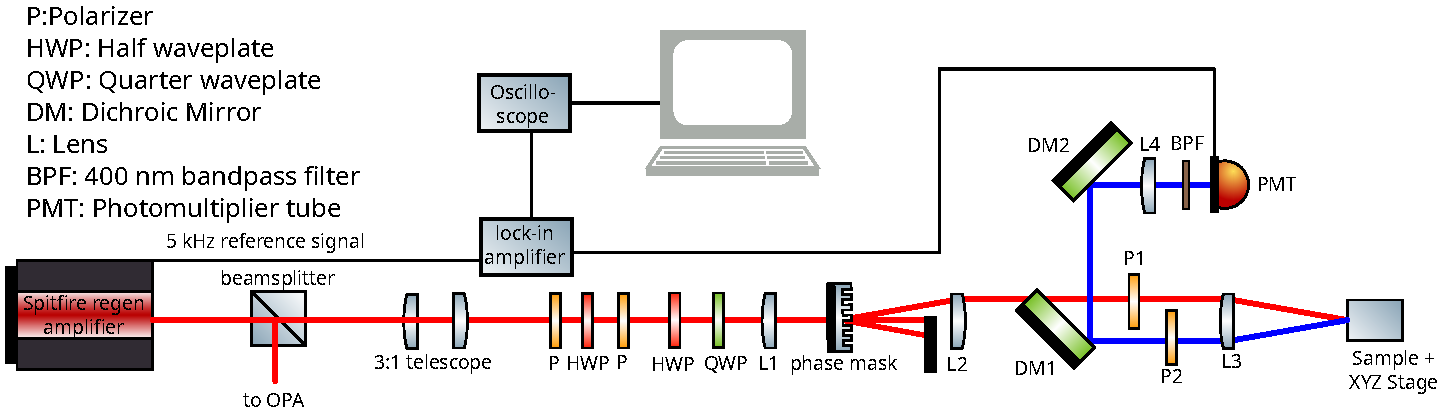
\includegraphics[width=\textwidth]{gfx/ch3/pdf/setup.pdf}
\caption{\label{fig:setup}Schematic drawing of the \gls{shg} setup used in this research. After \citet{morey_automated_2024}.}
\end{figure}

Finally, the polarized output reflects off of two dichroic mirrors (oriented in such a way as to cancel the differing effect of the Fresnel equations on the reflectivity of S and P polarized light) and is focused through a $400$ \si{nm} bandpass filter onto a \gls{pmt} by a $400$ \si{mm} lens.
The current output of the \gls{pmt} is filtered by a lock-in amplifier (for static \gls{shg}, set to the $5$ \si{kHz} repetition rate of the laser) and read out on an oscilloscope.
The phase mask, incoming polarizer, and outgoing polarizer are mounted on rotating lens tubes which are connected via pulley to a common motor shaft driven by a brushless DC motor.
The motor thus continuously rotates the plane of incidence of the experiment, since the latter is entirely defined by the phase mask and the polarizers.
The rotation angle is tracked as a function of time by an optical rotary encoder, consisting of a laser pointer passed through a chopper wheel (with 100 slots) mounted at the end of the motor shaft and detected via photodiode.
The encoder signal and the lock-in signal are both sent to a homemade oscilloscope (an Arduino Uno microcontroller which separates the lock-in signal into different individual rotations by looking for peaks in the encoder signal), the output of which is sent to a computer for further data processing.

\section{Before you build}\label{sec:beforeyoubuild}

I list here a few essential aspects of \gls{shg} that should be considered before designing a new setup.

\subsection{Spot size}

One of the most important quantities in an \gls{shg} setup is the diameter of the probe spot.
Ideally, this diameter is as small as possible, so as to measure the smallest samples or domain sizes.
However, there is an important caveat: for constant fluence (i.e. supposing we are limited by the sample damage threshold), the \gls{shg} signal to noise ratio scales linearly in the area excited by the probe, and thus \gls{shg} microscopes have a difficult time measuring small \gls{shg} signals compared to traditional \gls{shg} setups with a larger excitation area.
To see this, let us say that our detector measures the number of photons per \gls{shg} pulse, which is proportional to the pulse energy $U_p(2\omega)$.
Assuming the input and output pulse intensity profiles have the shape of a square wave with width $\tau$ and height $I_p(\omega)$ and $I_p(2\omega)$, respectively, we have
\begin{equation}
U_p(2\omega) = A I_p(2\omega) \tau
\end{equation}
and
\begin{equation}
U_p(\omega) = A I_p(\omega) \tau
\end{equation}
where $A$ is the area of the beam at the sample surface.
The \gls{shg} intensity is proportional to the square of the input intensity
\begin{equation}
I_p(2\omega) \propto I_p^2(\omega)
\end{equation}
so that
\begin{equation}
U_p(2\omega) \propto \frac{U_p^2(\omega)}{A\tau}.
\end{equation}
Substituting for the fluence $f$
\begin{equation}
f(\omega) = \frac{U_p(\omega)}{A}
\end{equation}
we have
\begin{equation}
U_p(2\omega) \propto \frac{f^2(\omega)A}{\tau}
\end{equation}
i.e., if we hold the fluence constant at the sample damage threshold, the number of photons in the generated \gls{shg} pulse is proportional to the excitation area and inverse to the pulse width.
The signal to noise ratio is then given by
\begin{equation}
\mathrm{SNR} \propto \frac{U_p(2\omega)}{\sqrt{r}}
\end{equation}
where $r$ is the system repetition rate.

\subsection{Oblique vs. normal incidence}

While all of the results presented in this thesis utilized the setup in \cref{fig:setup}, where the incident beam makes a small angle with respect to the sample normal, plenty of groups use a different approach where that angle is set to $0^\circ$.
This has the obvious disadvantage of not specifying all of the tensor elements, since any element $\chi_{ijk}$ with $i, j, k = z$ is not accessible in this geometry.
However, in some cases this can actually be something of an advantage.
For example, sometimes unwanted \gls{shg} contributions (see \cref{sec:manyshgterms}) may be avoided in the normal incidence geometry, assuming the \gls{na} of the focusing optic is small enough that longitudinal components of the electric field are nearly zero.
Furthermore, in some materials the order parameter only couples to one or two elements of $\chi_{ijk}$; if none of these elements have a $z$ index, it is needless to complicate the analysis with oblique incidence.

In my experience, oblique incidence seems to be useful in two broad cases.
For one thing, some order parameters only show up in the $z$ components of $\chi_{ijk}$ (this is the case in \tastwo, see \cref{sec:tastwo}), in which case one obviously needs a nonzero angle of incidence to access these components.
A more subtle point is that, even if in practice all of the phenomenology of a particular sample only shows up in the $x$ and $y$ indices of $\chi_{ijk}$, still one must measure the full tensor to \emph{rule out} unseen phenomenology in the other indices.
Both the \ce{CaMn2Bi2} (\cref{ch:ch5}) and \ce{CuBr2} (\cref{ch:ch6}) works presented in this thesis are examples of exactly this point, where the main scientific arguments involve either comparing \gls{shg} patterns in two domains or comparing oscillation amplitudes in different polarization channels.
Clearly one needs to know all of the tensor elements to make those arguments exact.

\chapter{Automated Polarization Rotation for Multi-Axis Rotational-Anisotropy Second Harmonic Generation Experiments}\label{ch:polrotators}
\section{Preface}

This chapter is based on a manuscript intended for standalone publication and modified to fit the format of this thesis.
It was coauthored by myself and Karna Morey (as co-first authors), along with Baiqing Lv, Zongqi Shen, and Nuh Gedik.
Karna Morey and I initiated the project, designed and built the polarization rotators, performed the demonstration experiment, and wrote the paper.
Baiqing Lv and Zongqi Shen contributed to the design and helped review the manuscript.
Nuh Gedik supervised the project.

\section{Abstract}

\gls{rashg} is a nonlinear optical technique used to probe the symmetry of condensed matter systems. 
Measuring the dependence of the SHG susceptibility on one or more external parameters, notably strain, field, temperature, or time delay, is an extremely powerful way to probe complex phases of quantum materials. 
Experimentally, extracting maximal information about the SHG susceptibility tensor requires measurements of S and P polarized input and output combinations, which naturally involves the rotation of the polarizers during data collection.  
For multi-axis experiments, this has proved challenging since polarization rotation is typically done manually. 
Automating this process eliminates labor constraints, reduces uncertainty due to low-frequency noise, and expands the type of multi-axis datasets that can be collected; however, it is difficult due to geometrical constraints within the setup.
In this work, we design and implement low-cost, high-fidelity automated polarization rotators for use in multi-axis \gls{rashg}.
These polarization rotators utilize an electrical slip ring to transfer power to the rotating \gls{rashg} optical setup as well as a miniature stepper motor to perform the polarization rotation.
We demonstrate this automated system in time-resolved \gls{rashg} measurements in the non-centrosymmetric semiconductor \ce{GaAs}. 
For the multi-axis measurements described above, this automated system permits data averaging over longer periods, vastly expedites data collection, and expands the setup measurement capability.
This ultimately opens new frontiers in probing quantum materials using multiple tunable external parameters.

\section{\label{km-sec:intro} Introduction}

Probing the structure of crystalline solids is essential to understanding their intrinsic functionalities. 
Traditionally, diffraction techniques based on the scattering of e.g. x-rays are used to determine this structure; however, these techniques predominantly measure the total electron density and are thus insensitive to long-range ordering of the valence electron subsystem.
In contrast, nonlinear scattering techniques at optical frequencies like \gls{rashg} are sensitive rather to the total charge density, and thus offer a complementary view of the electronic, magnetic, and lattice properties of quantum materials \citep{torchinsky_low_2014, fichera_second_2020}.\footnote{In this paper, we discuss \glsfmtshort{rashg}, although the results are fully generalizable to arbitrary harmonics, e.g. third harmonic generation.}


Furthermore, due to the non-invasive nature of \gls{rashg}, it can also be used to investigate changes along one or more measurement axes, such as strain, field, pressure, temperature, or time delay.
The phase diagram of quantum materials is heavily influenced by these independent variables, and thus, changes to the SHG response along such measurement axes are of great interest.
For example, previous studies have used various continuous experimental parameters such as pressure \citep{li_high-pressure_2022}, time delay\citep{shan_giant_2021}, and magnetic field to investigate phase transitions in quantum materials.
Such measurements can illuminate the roles that charge, spin, and thermal degrees of freedom play within quantum materials.

Second harmonic generation gleans microscopic information through the coupling of an order parameter to the second harmonic susceptibility tensor (at least a third-rank tensor with 18 independent components) \citep{boyd}. 
This tensor governs the relationship between the vector properties (i.e. polarization and intensity) of the incident radiation and the generated second harmonic, as shown in \cref{km-eq:intensity}.
The complexity of this tensor means that a significant amount of data is needed to fully resolve the tensor components, posing experimental challenges with data collection.
The importance of resolving the tensor components can be seen by considering Neumann's principle, which states that these tensors must be invariant under symmetry operations of the material's point group, which constrains the tensors' independent and nonzero elements \citep{birss}. 
By measuring the intensity and polarization of the generated second harmonic radiation, \gls{rashg} provides information about these tensor elements and thus the underlying point group.
When performing experiments with more than one measurement axis, the data constraints mentioned above can often be especially burdensome, limiting the type of experiments that can be performed using \gls{rashg}.
Thus, new methods for collecting data efficiently for multi-axis \gls{rashg} experiments are incredibly important.

\begin{figure}
\centering
\phantomsubfloat{\label{km-fig:1a}}
\phantomsubfloat{\label{km-fig:1b}}
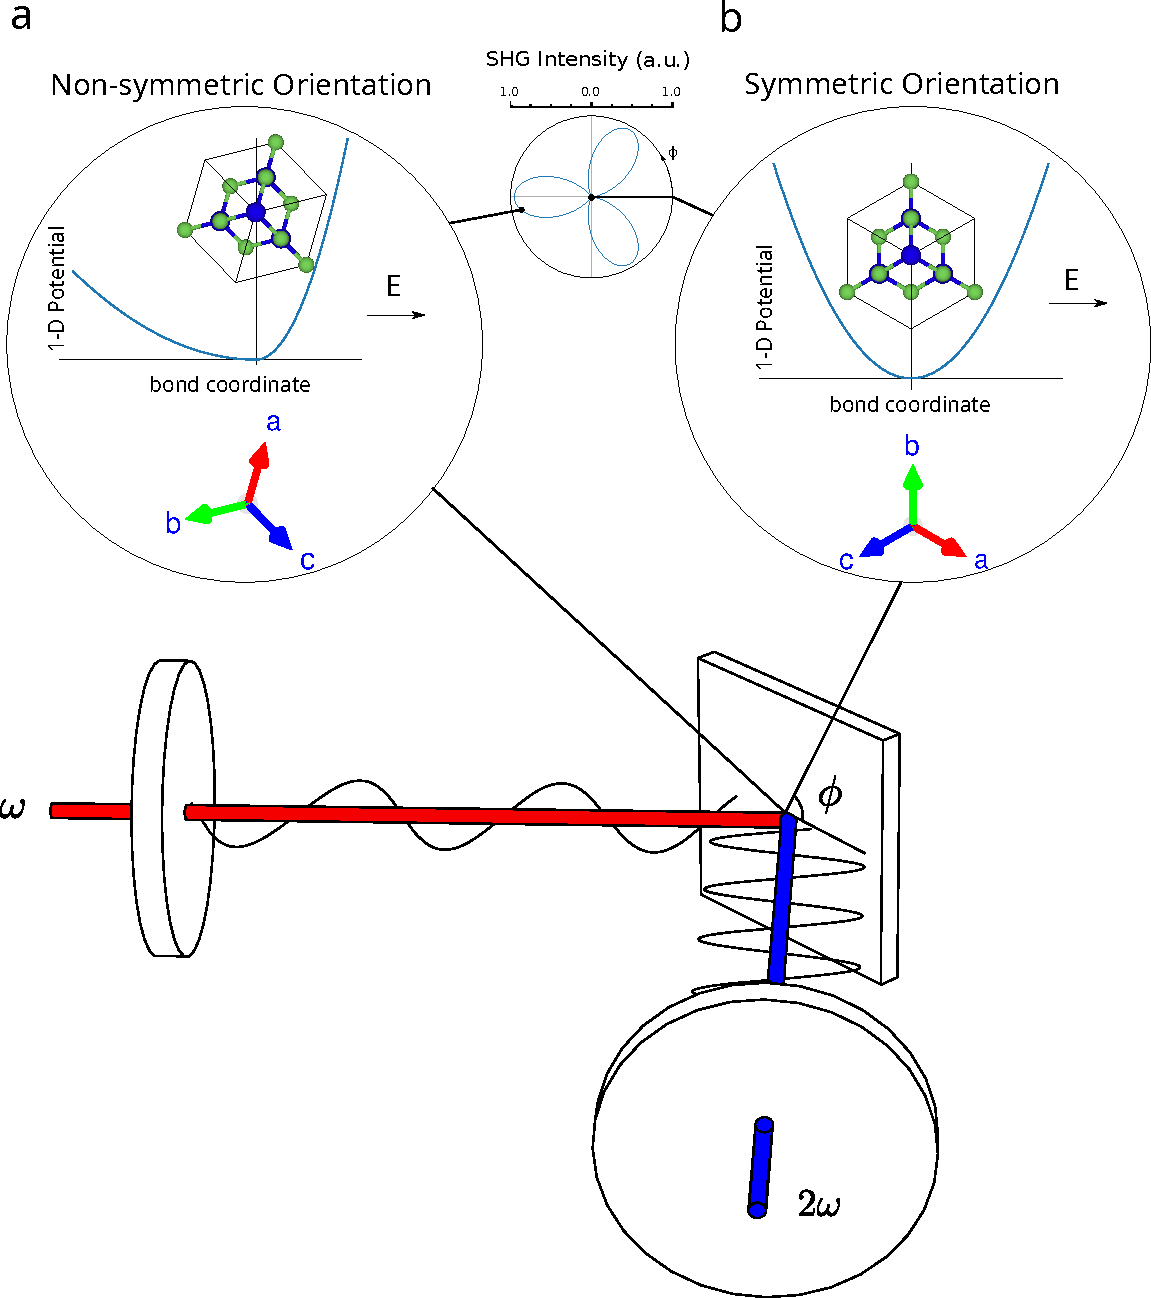
\includegraphics[width=0.8\textwidth]{gfx/ch4/km-fig1.pdf}
\caption[A demonstration of \glsfmtshort{rashg} in the test sample \ce{GaAs}]{
\label{km-fig:1}
\begin{enumerate*}[label=\caplabel, ref=\capref]
\item[] A demonstration of \glsfmtshort{rashg} in the test sample \ce{GaAs}.
\qty{800}{nm} light comes in at an oblique angle of incidence, after being passed through a polarizer.
The polarization axis of the light is in the plane of incidence and is denoted in the insets of the figure with a black arrow.
Depending on the angle of the plane of incidence relative to the crystallographic axes, as well as the polarization of the beam relative to that incoming plane of incidence, the second harmonic response to the stimuli should vary from zero points (nodes) to non-zero maxima.
\end{enumerate*}
}
\end{figure}

A more detailed understanding of the information that needs to be collected to fully resolve the second harmonic susceptibility can be seen by considering \cref{km-fig:1}.
\Cref{km-fig:1} shows a schematic of an \gls{rashg} setup, where near-infrared light from the laser source enters at oblique incidence and is scattered off the front of the sample, generating blue light at the second harmonic frequency.
To leading order, the measured second harmonic intensity is given by
\begin{equation}
I(\phi) = \big| E^{\mathrm{out}}_i(\phi) \chi^{(2)eee}_{ijk} E^{\mathrm{in}}_j(\phi) E^{\mathrm{in}}_k(\phi)\big|^2,
    \label{km-eq:intensity}
\end{equation}
where $\phi$ is the azimuthal angle between the crystallographic axes and the plane of incidence, $E^{\mathrm{out}}$ and $E^{\mathrm{in}}$ are the polarization vectors of the outgoing and incoming light, respectively, and $\chi^{(2)eee}$ is the SHG electric-dipole susceptibility tensor.
For certain values of $\phi$, as shown in \cref{km-fig:1a}, the sample is symmetric with respect to the polarization axis of the incoming light; in this case, the second harmonic generation is constrained to be zero, whereas in general arbitrary angles give a non-zero second-harmonic response (see \cref{km-fig:1b}).
Neumann's principle dictates that \cref{km-eq:intensity} captures the symmetry considerations shown in \cref{km-fig:1}, i.e. the symmetries of the crystal are embedded into its nonlinear susceptibility tensor $\chi^{(2)}$.

These considerations demonstrate the necessity of measuring the full rotational anisotropy of the SHG response, as well as its dependence on the incoming and outgoing polarization directions (which may be P or S-polarized, leading to four independent polarization channels).
The former requires rotating the plane of incidence, which is typically done by rotating the optical setup itself rather than the sample \citep{petersen_nonlinear_2006,torchinsky_low_2014, fichera_second_2020, camn2bi2}. 
The geometric constraints involved in rotating the optical setup make it challenging to use electromechanical components to rotate the polarizers shown in \cref{km-fig:1} between S and P configurations, since naively it is difficult to transfer power to the rotating frame of reference.
Because of this, switching between different polarization channels is typically done manually, resulting in time and labor constraints that often limit data collection beyond a single polarization combination \citep{shan_giant_2021}.
Such constraints severely restrict the ability to infer tensor elements from the \gls{rashg} data and limit RA-SHG to studies involving often just a single tuning parameter. 

Previous multi-axis \gls{rashg} studies typically either collected exclusively one polarization channel \citep{shan_giant_2021} (for more than one axis) or simply sacrificed the quantity of collected data and therefore inferred statistics. 
However, these approaches can often miss certain features in \gls{rashg} data that would be apparent if more efficient data-taking methods were available.
For example, phase transitions in which the order parameter couples differently to different polarization channels through the second harmonic susceptibility \citep{camn2bi2} are best characterized by taking the full rotational anisotropy data.
The benefit of collecting all four polarization combinations underscores the appeal of automated polarization control of \gls{rashg} setups.

\begin{figure}
\centering
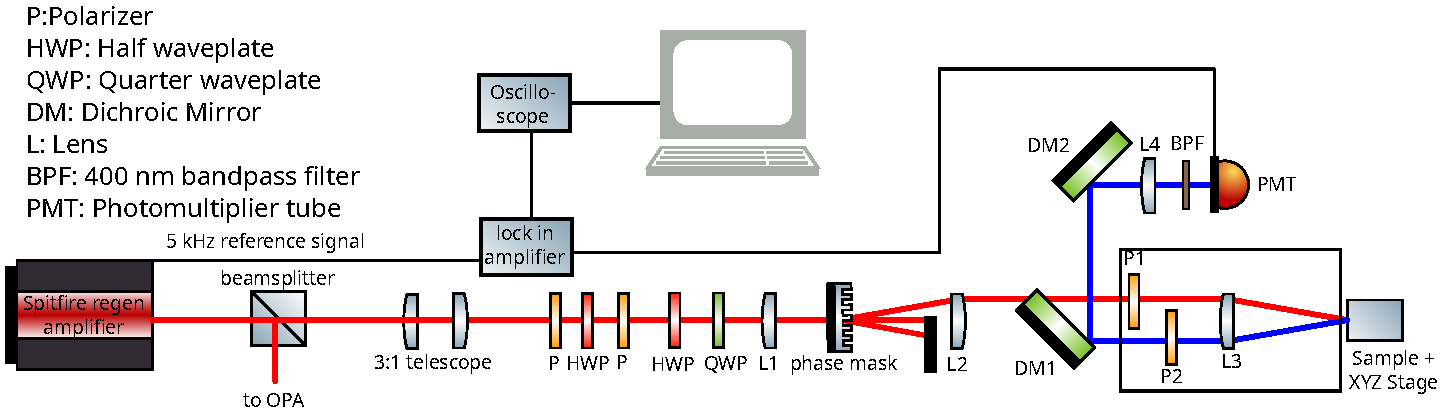
\includegraphics[width=\textwidth]{gfx/ch4/km-fig2.pdf}
\caption[A diagram of the full second harmonic generation setup]{
\label{km-fig:2}
\begin{enumerate*}[label=\caplabel, ref=\capref]
\item[] A diagram of the full second harmonic generation setup developed and described in \citet{fichera_second_2020}.
Boxed in part of the setup shows the area of interest of this work, where the incoming and outgoing polarization channels are set.
\end{enumerate*}
}
\end{figure}

In this work, we design and implement automated polarization rotators for use in multi-axis \gls{rashg} measurements. 
The devices utilize a miniature stepper motor housed in an electrical slip ring to circumvent the geometrical constraints imposed by the rotating plane of incidence.
In section \ref{km-sec:disc}, we discuss the specific application of automated polarization rotation to time-resolved RA-SHG and show that it not only expedites data collection but also reduces the setup's sensitivity to low-frequency noise. 
The advantages afforded by the automated polarization rotators exist not only for time-resolved measurements but for any measurements where an external parameter is being varied and compound rapidly as multiple parameters are varied at the same time.

\section{Design}
\label{sec:des}

A detailed schematic of the \gls{rashg} setup is shown in figure 2.
Telescoped pulses from a \qty{5}{kHz} pulsed regenerative amplifier (Spectra-Physics Spitfire) are attenuated using a half-waveplate set between two polarizers and then elliptically polarized using a half-waveplate and quarter-waveplate in series. 
The light is then focused by a lens onto a rotating phase mask (which separates the beam into different diffraction orders), and a beam block selects the +1 order beam which is then collimated using another lens (L2).
Finally, the beam passes through a dichroic mirror and a polarizer (P1) before being focused by a third lens (L3) onto the sample.
The reflected radiation is passed through an analyzer (P2) and is redirected using a dichroic mirror periscope, which has equal reflectivity for S and P-polarized light and selects exclusively the \qty{400}{nm} reflected radiation.
The two polarizers (P1 and P2) and the phase mask are mounted on a rotating shaft coupled to an optical rotary encoder.
After the dichroic mirrors, the second harmonic radiation is focused by a final lens (L4) onto a \qty{400}{nm} bandpass filter and photomultiplier tube.
The signal from the photomultiplier tube is sent to a lock-in amplifier synced to the \qty{5}{kHz} pulsed laser reference signal and the amplified signal is then correlated with the signal from the optical rotary encoder using a home-built oscilloscope. 

Importantly, the geometrical constraints introduced by the rotating plane of incidence mean that rotating P1 and P2 between S and P configurations electromechanically is challenging, as power must be transmitted from the stationary laboratory frame to electrical components lying in the rotating frame.

To solve this problem, we utilize a hollow-bore electrical slip ring and a miniature stepper motor, shown in an exploded-view diagram in \cref{km-fig:3a}.
A slip ring uses stationary conductive brushes sliding against a rotating through-bore cylinder to transfer power from a stationary reference frame to a rotating one, as shown in \cref{km-fig:3b} \citep{argibay_asymmetric_2010}. 
To accommodate the further requirement that the beams pass through the entire device unimpeded, we employ an \qty{8}{mm} stepper motor that fits in between the two beams.
\Cref{km-fig:3c} and \cref{km-fig:3d} show a front view of the device, with the wire grid polarizer in the P and S positions, respectively, and the polarization direction of the polarizer shown in arrows on the edge of the polarizer.
A full rendering, to scale, of the automated system within the full setup is shown in \cref{km-fig:6}. 

\subsection{Slip Ring}

Slip rings are a standard electromechanical device for transferring power from a stationary assembly to a rotating assembly.
An inner, rotating part of the slip ring can freely rotate relative to an outer, stationary part without compromising signal or power transmission.
This functionality is enabled by low-friction metal brushes that slide against another set of electrical contacts, allowing free rotation while maintaining good electrical conductivity \citep{argibay_asymmetric_2010}, as shown in \cref{km-fig:3b}.
To allow for the uninterrupted passage of the beams through the device, we use a hollow-bore slip ring (Moflon MT3899-S040-VD) whose \qty{38}{mm} inner bore rotates along with the lens tube-pulley assembly shown in \cref{km-fig:6}.
Either set screws located on the front side of the slip ring (as shown in \cref{km-fig:3}) or a 3D-printed cylindrical hollow bore adapter (not shown) can secure the inner bore of the slip ring to the lens tube.

\begin{figure}
\centering
\phantomsubfloat{\label{km-fig:3a}}
\phantomsubfloat{\label{km-fig:3b}}
\phantomsubfloat{\label{km-fig:3c}}
\phantomsubfloat{\label{km-fig:3d}}
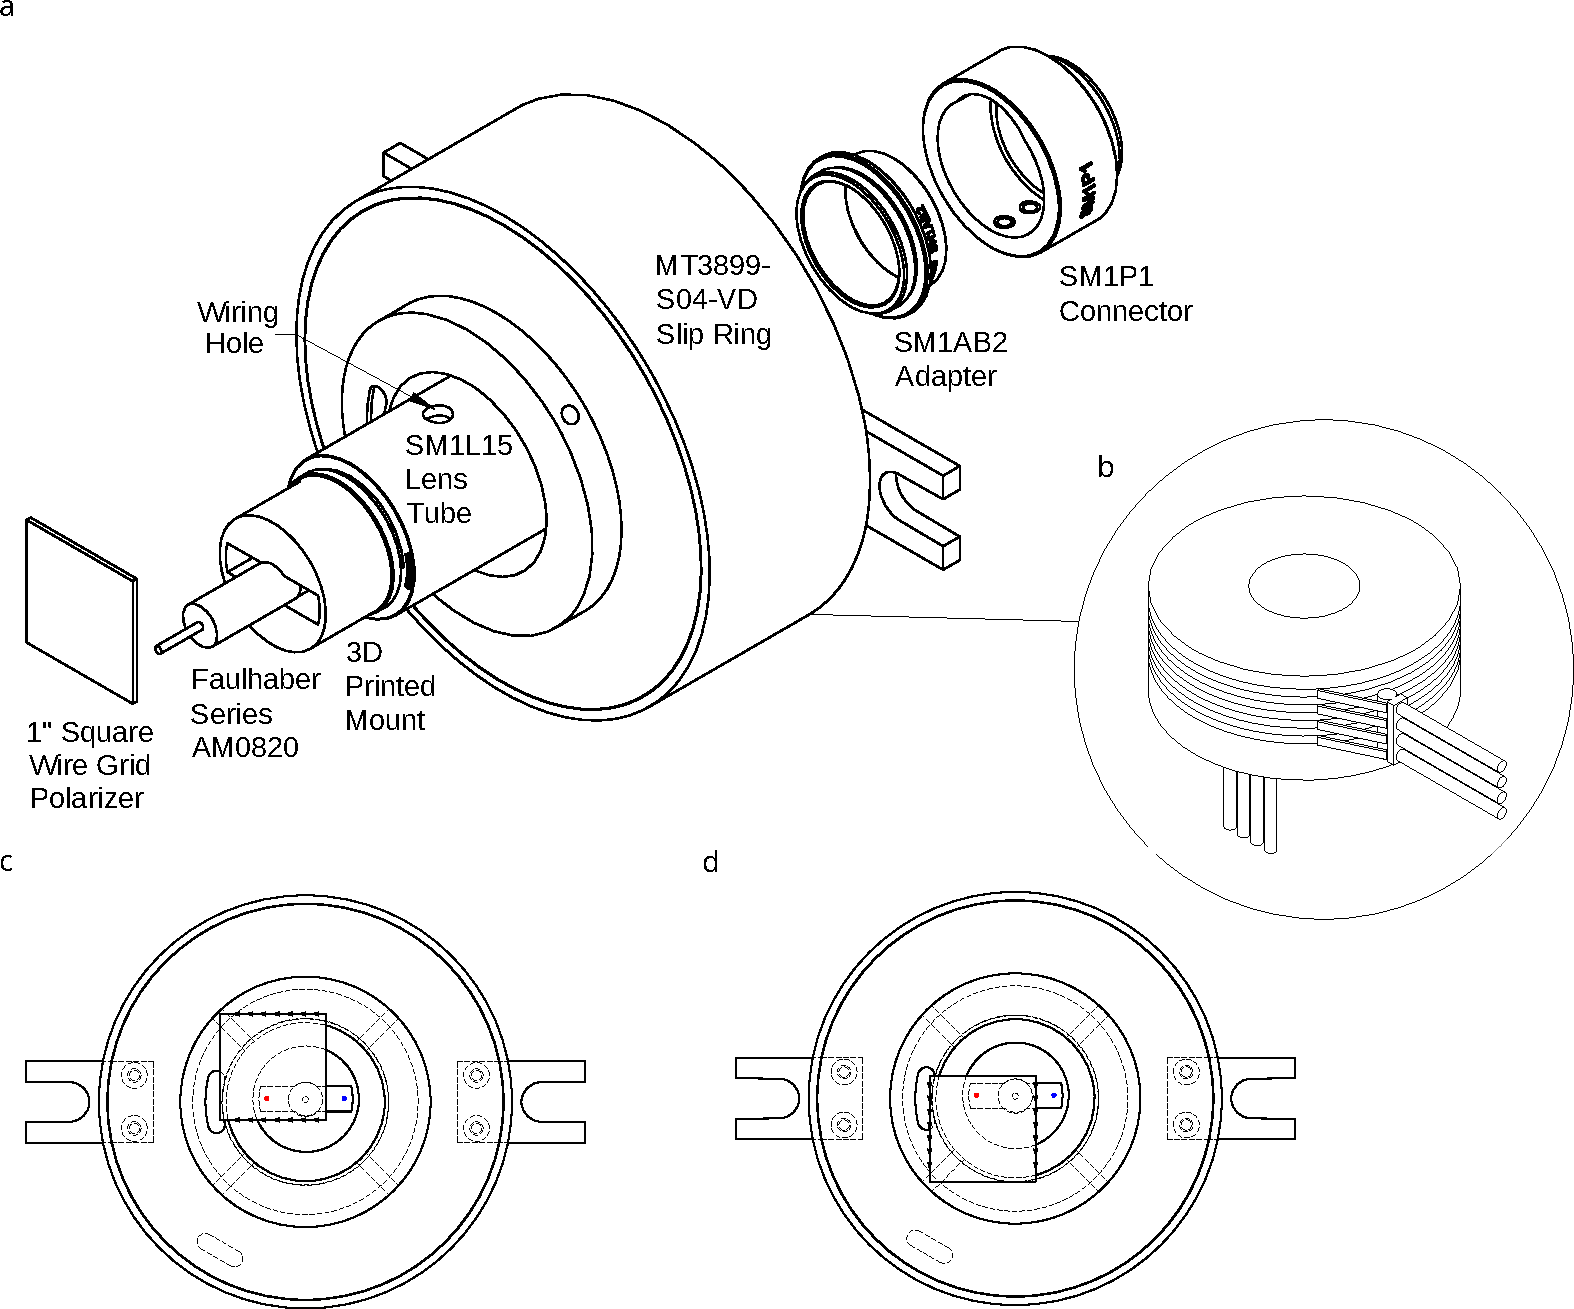
\includegraphics[width=\textwidth]{gfx/ch4/km-fig3.pdf}
\caption[Exploded-view diagram of one of the automated polarization rotators]{
\label{km-fig:3}
\begin{enumerate*}[label=\caplabel, ref=\capref]
\item An exploded-view diagram of one of the automated polarization rotators, with the individual components labeled.
Each of these is a manufactured part except for the 3D-printed mount.
\item A schematic of the interior of an electrical slip ring, where low-friction metal brushes allow for electrical conduction across a rotating assembly.
\item A front view of the device, in the P-polarized state, with arrows on the edge of the polarizer indicating the polarization direction.
\item Same as \cref{km-fig:3c}, but in the S-polarized state.
\end{enumerate*}
}
\end{figure}

\subsection{Miniature Stepper Motor}
\label{km-sec:stepper}
The hollow bore slip ring allows for the transfer of power to the rotating shaft.
To rotate the wire grid polarizer between S and P configurations while also allowing both beams to pass through the entire device, we use an \qty{8}{mm} diameter Faulhaber Series AM0820 stepper motor.
The stepper motor's shaft is epoxied to a \qty{1}{inch} square wire-grid polarizer roughly \qty{5}{mm} from the closest horizontal and vertical edges, as shown in \cref{km-fig:3c} and \cref{km-fig:3d}.
The stepper motor is mounted in the center of the SM1L15 lens tube using a custom, 3D printed mount as shown in \cref{km-fig:3a}. 
This mount, along with careful epoxying of the polarizer to the motor shaft, ensures that the incidence angle of the beam is close to normal.
Furthermore, the mount ensures that the stepper motor's shaft is aligned closely to the central rotation axis of the entire assembly, minimizing torques on the motor and polarizer.
This stepper motor can support up to \num{800} total micro-steps per revolution (\ang{0.45} per micro-step) and \qty{0.65}{mNm} of holding torque, and is small enough to fit in between the incoming and outgoing beams. 

The motor can then move the polarizer between the P configuration (\cref{km-fig:3c}) and the S configuration (\cref{km-fig:3d}) without manual intervention or the need to stop the rotation of the entire assembly.
The offset placement of the polarizer on the motor shaft allows only one of the beams (either incoming or outgoing) to pass through the polarizer.
The SM1AB2 and SM1P1 adapter pieces allow for arbitrary rotation relative to the longer lens tube-pulley assembly, allowing the beams to be aligned with the empty spaces in the stepper motor mount.
These adapter pieces also allow for small ($\pm \ang{20}$) rotations of the polarizer about the central axis to account for factory defects which may cause the polarization axis to be misaligned with the straight edges of the polarizer.

\begin{figure}
\centering
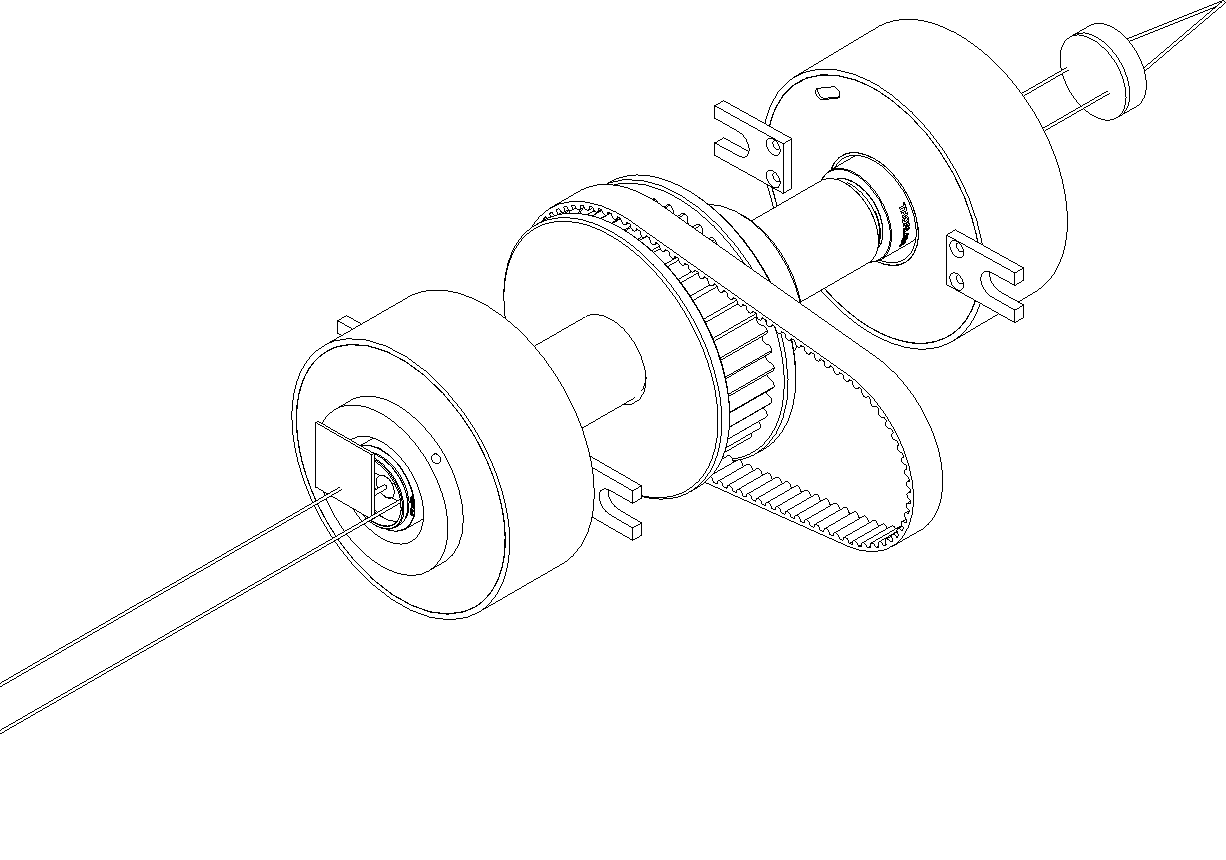
\includegraphics[width=\textwidth]{gfx/ch4/km-fig4.pdf}
\caption[A 3-dimensional rendering of the automated polarization rotators]{
\label{km-fig:6}
\begin{enumerate*}[label=\caplabel, ref=\capref]
\item[] A 3-dimensional rendering of the boxed-in part of the setup in \cref{km-fig:2}, with fully automated polarization rotators.
\end{enumerate*}
}
\end{figure}

Another copy of the same system shown in \cref{km-fig:3} is mounted on the other side of the lens tube-pulley assembly and controls the polarization of the reflected beam, as shown in \cref{km-fig:6}. 
The back sides of both devices, shown in \cref{km-fig:6}, are attached to the rotating lens tube-pulley-motor-shaft assembly shown in \cref{km-fig:6} via threads on the long central lens tube. 
A hole drilled in the top and bottom of the SM1L15 piece in each device shown in figure \cref{km-fig:3a} allows feedthrough wires to connect the four leads of the stepper motor to the four rotating inner-bore slip ring leads.
The four leads on the stationary side of each slip ring directly connect to a Geckodrive G250X digital step driver for each device, controlled by a single Arduino Nano Every.
This control circuit allows for the integration of the stepper motors with existing instrumentation software.

Whenever the stepper motors lose power, the polarizers need to be re-aligned due to the loss of their holding torque.
The alignment is performed by using a reference polarizer with a known polarization axis.
First, the plane of incidence of the entire assembly is positioned to the known polarization plane of the reference polarizer, then the polarizers themselves can be oriented by placing the beam through the reference polarizer and rotating the stepper motor until beam extinction (yielding an S-polarized alignment).  
The polarizers can then freely rotate between this S-polarized position and the orthogonal P-polarized position.

\section{Validation and Discussion}
\label{km-sec:disc}

\begin{figure}
\centering
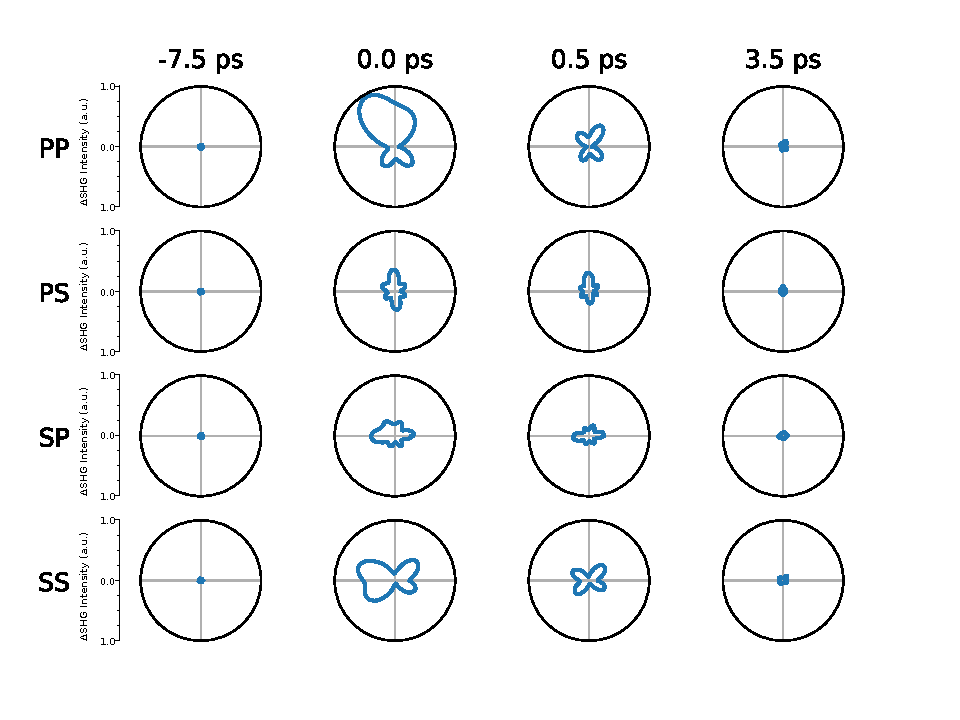
\includegraphics[width=\textwidth]{gfx/ch4/km-fig5.pdf}
\caption[Demonstration of the automatic polarization rotators]{
\label{km-fig:4}
\begin{enumerate*}[label=\caplabel, ref=\capref]
\item[] A polar plot of the change in SHG intensity (from the pre-pump state) as a function of time since zero-delay for the test sample GaAs.
This is a demonstration of using the automated polarization rotators to take \gls{trshg} data.
\qty{55} different pump-probe delays (only four time delays are plotted) were taken in this dataset, meaning that \qty{220} polarization rotations were performed using the automated polarizers.
\end{enumerate*}
}
\end{figure}

To test these automated polarization rotators, we performed time-resolved RA-SHG on the non-centrosymmetric semiconductor \ce{GaAs} \citep{ducuing_observation_1963, torchinsky_low_2014}. 
A pump line was added to the setup shown in \cref{km-fig:2} by mounting a \ang{45} mirror onto L3 so that the pump beam may be reflected directly onto the sample. 
The pump pulse is produced by an optical parametric amplifier (Spectra-Physics Topas) tuned to a wavelength of \qty{1.3}{$\mu$ m}.
The pump line includes a delay stage, which controls the relative time delay between the pump and the probe pulses, and a chopper wheel, which reduces the effective repetition rate of the pump pulses to \qty{2.5}{kHz}. 
With the pump repetition rate of \qty{2.5}{kHz} and the probe repetition rate of \qty{5}{kHz}, locking in at a frequency of \qty{2.5}{kHz} produces a signal proportional to the change in the \gls{shg} intensity relative to equilibrium.
For time-resolved measurements on \ce{GaAs}, shown in \cref{km-fig:4}, \qty{55} different pump-probe delays were taken, resulting in \qty{220} different automatic rotations of the polarizers.
The data in \cref{km-fig:4} shows the change in the \gls{shg} intensity relative to equilibrium as a function of the pump-probe delay, for each of the polarization channels. 
The use of the polarization rotators in this validation measurement demonstrates their functionality and broad utility for multi-axis \gls{rashg} measurements.

This system was also used to expedite data collection in recent studies of time-resolved, temperature-dependent \gls{rashg} \citep{camn2bi2}.
This particular type of \gls{rashg} measurement demonstrates the general advantages of automated polarization control in multi-axis \gls{rashg} measurements.
To see this, note that if the rotation of the polarizers is performed manually, the best data-taking strategy involves taking the time dependence of one polarization channel in full before moving to the next. 
However, in the presence of low-frequency noise (due to e.g. fluctuations in the laser intensity), this is problematic as the different polarization channels will not be taken under equivalent conditions. 
In the automated case, in contrast, all polarization channels can be taken at each time delay. 
This greatly decreases the experiment's susceptibility to low-frequency noise and expedites data taking by allowing for overnight and multi-day scans.

Automated polarization rotation thus vastly improves RA-SHG data collection, eliminating the need for manual polarization rotation, especially in cases of multiple experimental axes. 
The roughly \qty{1,000}{\$} total cost of both devices (not including polarizers) makes them relatively inexpensive, and the design is easily implementable in existing \gls{rashg} setups.
Multi-axis measurements are becoming increasingly important to resolve complicated phase diagrams and competing orders, and thus future measurements will increasingly rely on automated systems such as the one presented in this work.

\chapter{Second harmonic generation as a probe of broken mirror symmetry in 1\textit{T}-\ce{TaS2}}\label{ch:tastwo}
\chapter{Light-induced reorientation transition in the antiferromagnetic semiconductor \ce{CaMn2Bi2}}\label{ch:cmb}
\chapter{Amplitude-mode electromagnon in the XXZ chain \ce{CuBr2}}\label{ch:cubr2}
\chapter{Concluding remarks}\label{ch:conclusion}

\backmatter*
\bibliography{fichera-bfichera-phd-physics-2024-source}

\end{document}
